% Note: loosely based on 2018 summer project report. Will fit it to department guidelines at the very end.
\documentclass[parskip=full, numbers=noenddot]{scrreprt}

\usepackage[english]{babel}
\usepackage[utf8]{inputenc}
\usepackage{csquotes}
\usepackage[backend=biber, doi=false, isbn=false, url=false, date=year]{biblatex}
%\addbibresource{mainreport.bib}

\usepackage{graphicx}
  \graphicspath{ {./graphics/} }
\usepackage{subcaption}
\usepackage{url}
\usepackage{varioref}
\usepackage{tabularx}
  \newcolumntype{L}{>{\raggedright\arraybackslash}X}
\usepackage[version=4]{mhchem}
\usepackage{siunitx}
\DeclareSIUnit\molar{\mole\per\cubic\deci\metre}
\DeclareSIUnit\Molar{\textsc{m}}
\usepackage{booktabs}
\usepackage{longtable}


\title{Quantifying the bias in SELEX procedure}
\author{Candidate number XXXXX}

\begin{document}

\maketitle
% Will deal with the intricacies of the cover pages at the very end.

\begin{abstract}
 
Abstract.
 
\end{abstract}

\tableofcontents

\chapter*{List of Abbreviations}
\label{ch:abbrev}

\chapter{Introduction}
\label{ch:intro}

Introduction.

\chapter{Results}
\label{ch:results}

\section{Nucleosome EMSA SELEX}
\label{sec:resultemsaselex}

To study the effect of CpG and non-CpG methylation on the sequence specificity in the nucleosome, I carried out four cycles of EMSA SELEX. The input library (lig147) contained 147-base pair DNA ligands with 101 random base pairs at the centre flanked by i5 and i7 barcoding sequences. In each cycle of EMSA SELEX, the DNA ligands were reconstituted with Xenopus laevis histone octamers. Then, EMSA was conducted to separate naked DNA and DNA bound to histone octamers. This allowed DNA with sequences most conducive to nucleosome reconstitution to proceed to the next cycle.

The experiment was divided into four groups: plain DNA, CpG-methylated DNA, DNA with all cytosines methylated (all-C-methylated DNA), and DNA with half of its cytosines methylated (half-C-methylated DNA).

\subsection{DSSYNV2 was able to correctly amplify lig147 and methylated ligands}
\label{ssec:amplig}

% Delete this paragraph. This is more appropriate in the methods section and is repeated there.
First, lig147 was amplified using a theromocycling protocol modified from that for Phusion High-Fidelity DNA Polymerase (ThermoFisher, F530L). For all-C-methylated DNA, cytosines in the dNTP mix were replaced by 5-methylcytosines in the initial amplification step. For half-C-methylated DNA, half of the cytosines in the dNTP mix were replaced by 5-methylcytosines. CpG-methylation was carried out by adding M.SssI (CpG methyltransferase), S-adenosylmethionine, \ce{MgCl2}, and DTT to the input library, and incubating the mixture.

% Repeats figure captions
Gel electrophoresis of the products from all experimental groups yielded a strong band between 100 and 200 nucleotides (figure~\ref{fig:amplig}). Spectrophotometry showed that the DNA concentration after amplification lay within \SIrange{30}{40}{\nano\gram\per\micro\litre}, corresponding to the expected \SI{38}{\nano\gram\per\micro\litre}. These results suggest that the protocol successfully amplified lig147 and was also successful for the forms of methylation tested.

\begin{figure}[htpb]
  \centering
  \begin{subfigure}[htpb]{0.4\textwidth}
    \centering
    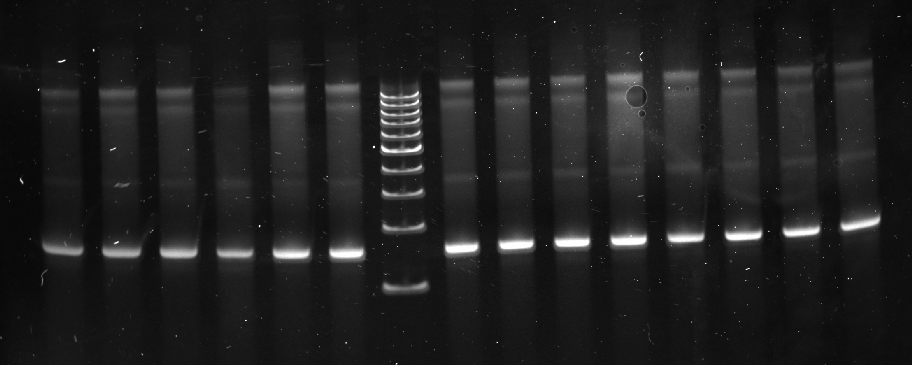
\includegraphics[width=\textwidth]{amplig_a}
    \caption{A}
    \label{fig:amplig_a}
  \end{subfigure}
  \begin{subfigure}[htpb]{0.4\textwidth}
    \centering
    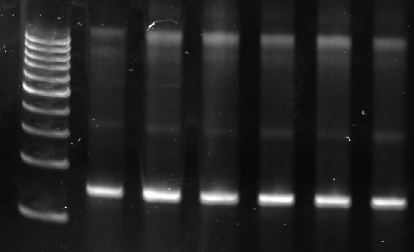
\includegraphics[width=\textwidth]{amplig_b}
    \caption{B}
    \label{fig:amplig_b}
  \end{subfigure}
  \begin{subfigure}[htpb]{0.4\textwidth}
    \centering
    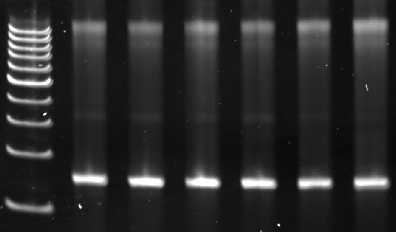
\includegraphics[width=\textwidth]{amplig_c}
    \caption{C}
    \label{fig:amplig_c}
  \end{subfigure}
  \begin{subfigure}[htpb]{0.4\textwidth}
    \centering
    
\includegraphics[width=\textwidth]{test}
    \caption{D}
    \label{fig:amplig_d}
  \end{subfigure}
  \caption{Gel electrophoresis in 8\% TBE gels for (A) amplified lig147 (B) half-C-methylated (C) all-C-methylated, and (D) CpG-methylated DNA. All lanes exhibited a strong band between 100 and 200 nucleotides. Slower-migrating fainter bands corresponded to single-stranded DNA as was expected.}
  \label{fig:amplig}
\end{figure}

\subsection{Two related protocols were able to reconstitute nucleosomes}
\label{ssec:reconstnuc}

% Delete or massively shorten this. Move details to methods section.
The input libraries generated for each experimental group were each subjected to four cycles of EMSA SELEX. In these cycles, the DNA ligands were reconstituted with histone octamers with octamer:DNA ratios ranging from 1.48:1 to 0.09:1. The products were analysed using EMSA on 6\% DNA retardation gels to separate naked DNA from DNA bound as part of reconstituted nucleosomes. The DNA was then eluted and amplified for use as the input for the next EMSA SELEX cycle.

Two related variants of the EMSA SELEX protocol were tested. They were loosely based on Dyer (2004), and differed in the composition of the dilution buffer. The dilution buffer for one protocol included protease inhibitor, while the other did not.

EMSA in all cycles yielded strong bands corresponding to naked 147-base pair DNA. It also yielded bands corresponding to reconstituted nucleosomes that are fainter as the proportion of histone octamer decreased in the solution (figure~\ref{fig:reconstnuc}).
% Remove all references to the two variants of the reconstitution protocol.
These observations applied to both variants of the EMSA SELEX. These observations confirmed that nucleosome reconstitution protocols based on Dyer (2004) were successful, even for methylated DNA.
% This is discussion and should not be here.
I adhered to the protocol without protease inhibitor to generate products for subsequent procedures because

\begin{figure}[htpb]
  \centering
  \begin{subfigure}[htpb]{0.4\textwidth}
    \centering
    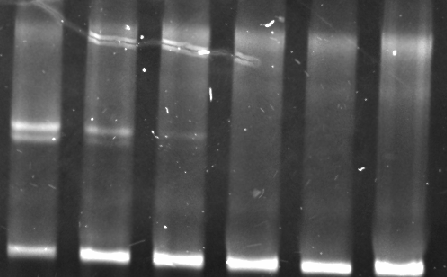
\includegraphics[width=\textwidth]{reconstnuc_a}
    \caption{A}
    \label{fig:reconstnuc_a}
  \end{subfigure}
  \begin{subfigure}[htpb]{0.4\textwidth}
    \centering
    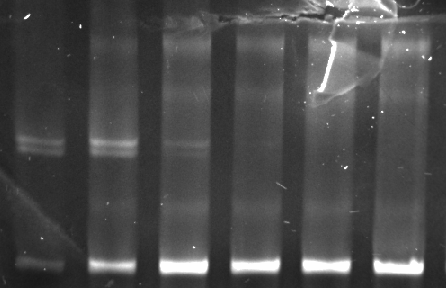
\includegraphics[width=\textwidth]{reconstnuc_b}
    \caption{B}
    \label{fig:reconstnuc_b}
  \end{subfigure}
  \begin{subfigure}[htpb]{0.4\textwidth}
    \centering
    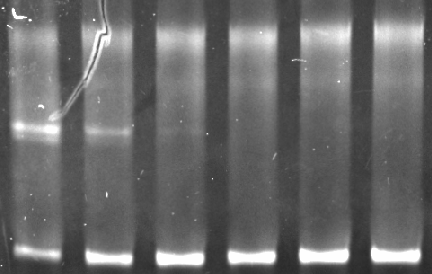
\includegraphics[width=\textwidth]{reconstnuc_c}
    \caption{C}
    \label{fig:reconstnuc_c}
  \end{subfigure}
  \begin{subfigure}[htpb]{0.4\textwidth}
    \centering
    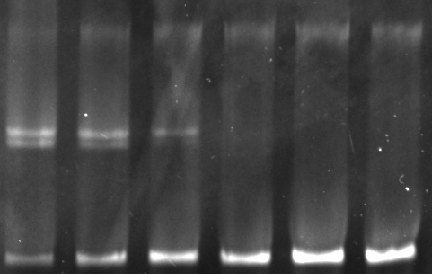
\includegraphics[width=\textwidth]{reconstnuc_d}
    \caption{D}
    \label{fig:reconstnuc_d}
  \end{subfigure}
  \caption{First cycle gel electrophoresis for EMSA in 6\% DNA retardation gels for (A) non-methylated DNA, (B) half-C-methylated (C) all-C-methylated, and (D) CpG-methylated DNA. Lanes for all images (left to right): (1) 1.48:1 histone octamer:DNA, (2) 0.74:1 histone octamer:DNA, (3) 0.37:1 histone octamer:DNA, (4) 0.19:1 histone octamer:DNA, (5) 0.09:1 histone octamer:DNA, and (6) DNA without histone octamer added. These results are representative for all cycles of EMSA SELEX.}
  \label{fig:reconstnuc}
\end{figure}

\subsection{Barcoding and subsequent PCR amplification worked}
\label{ssec:barcoding}

% No quantification of the concentrations of DNA needed here. Focus on sequencing.
Following elution of the DNA from EMSA in the four SELEX cycles, IDT barcodes were added for Illumina sequencing. The DNA elution products from each cycle of EMSA SELEX were used as templates. I tested the use of DreamTaq polymerase and Phusion DNA polymerase (both ThermoFisher) as DNA polymerase enzymes for barcoding.

% Debugging should probably be in a separate subsection in the results or discussion section
Gel electrophoresis of the products amplified by DreamTaq using recommended protocols yielded bands corresponding to 147 base pairs, suggesting that the amplification succeeded (figure~\ref{fig:barcoding_a}). However, gel electrophoresis of the products amplified by Phusion using recommended protocols did not yield this band (figure~\ref{fig:barcoding_b}).

Repeating the Phusion amplification using qPCR yielded saturation curves (figure~\ref{fig:qpcr}), suggesting that amplification indeed took place. As qPCR required a lower concentration of the template, it was hypothesised that Phusion initially failed because the ligand was too concentrated. Different DNA polymerases from different vendors are efficient with differing template concentrations – for example, DreamTaq requires ... while Phusion requires ... (citation needed). Therefore, I diluted the template DNA further by adding \SI{70}{\micro\litre} dilution buffer to each well. The resulting 8\% TBE gel yielded the band corresponding to 147 base pairs (figure~\ref{fig:barcoding_c}), confirming the hypothesis.

\begin{figure}[htpb]
  \centering
  \begin{subfigure}[htpb]{0.4\textwidth}
    \centering
    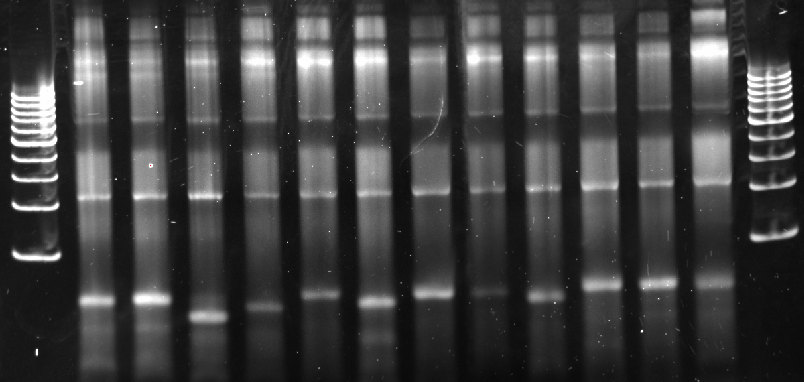
\includegraphics[width=\textwidth]{dreamtaq}
    \caption{A}
    \label{fig:barcoding_a}
  \end{subfigure}
  \begin{subfigure}[htpb]{0.4\textwidth}
    \centering
    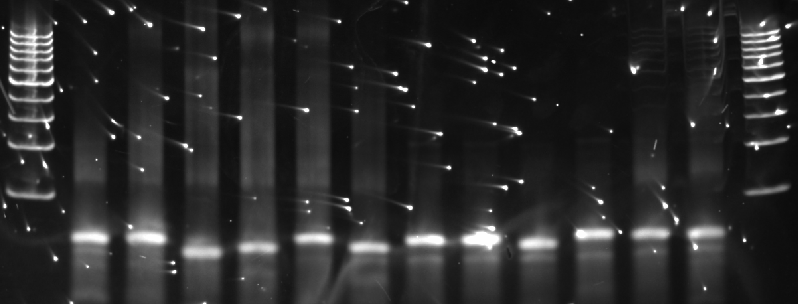
\includegraphics[width=\textwidth]{phusion_old_a}
    \caption{B}
    \label{fig:barcoding_b}
  \end{subfigure}
  \begin{subfigure}[htpb]{0.4\textwidth}
    \centering
    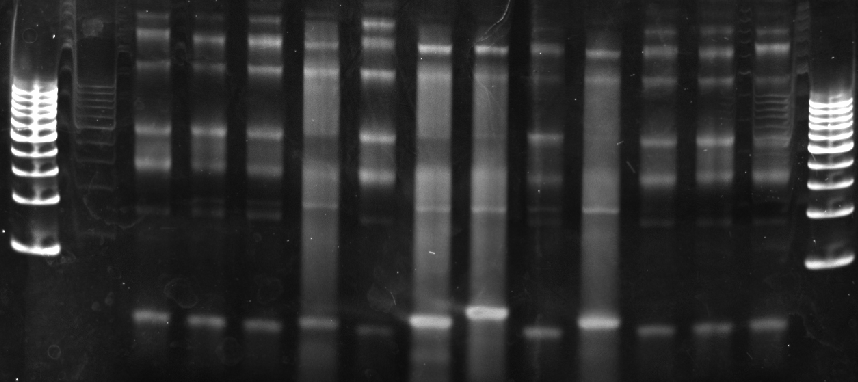
\includegraphics[width=\textwidth]{phusion_new_a}
    \caption{C}
    \label{fig:barcoding_c}
  \end{subfigure}
  \begin{subfigure}[htpb]{0.4\textwidth}
    \centering
    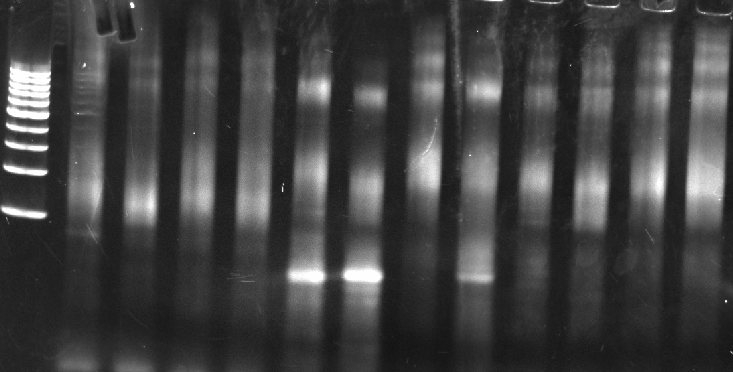
\includegraphics[width=\textwidth]{qpcrgel}
    \caption{D}
    \label{fig:barcoding_d}
  \end{subfigure}
  \caption{A - DreamTaq gel, B - old Phusion gels for rows A and B, C - new Phusion gels for rows A and B, D - qPCR gel}
  \label{fig:barcoding}
\end{figure}

\begin{figure}[htpb]
  \centering
  \begin{subfigure}[htpb]{0.3\textwidth}
    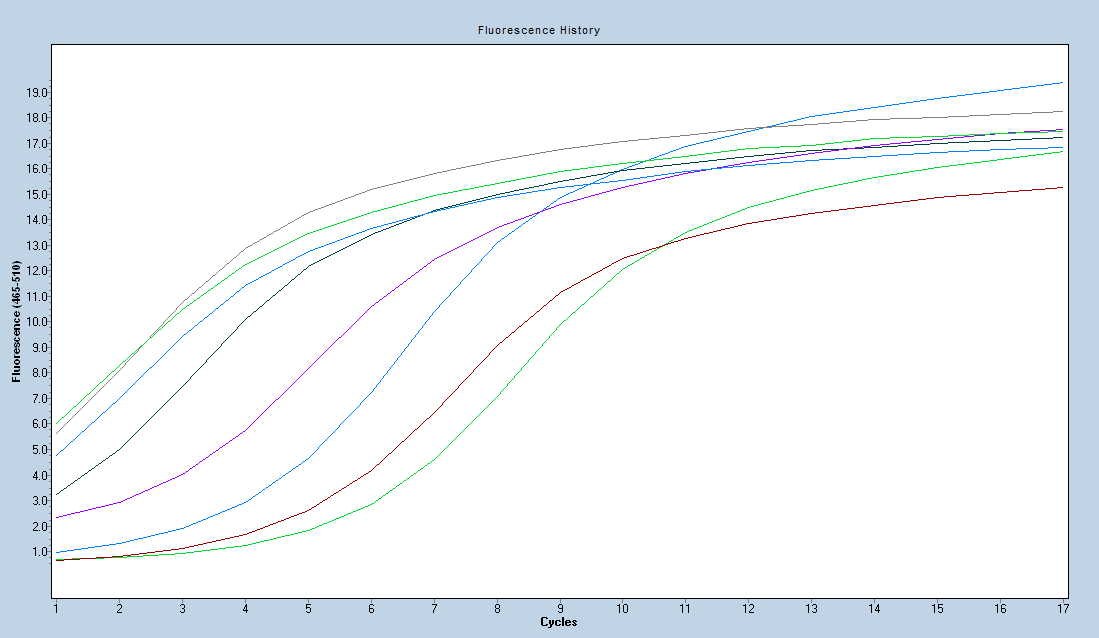
\includegraphics[scale=0.1]{qPCR_B}
    \caption{A}
    \label{fig:qpcr_a}
  \end{subfigure}
  \begin{subfigure}[htpb]{0.3\textwidth}
    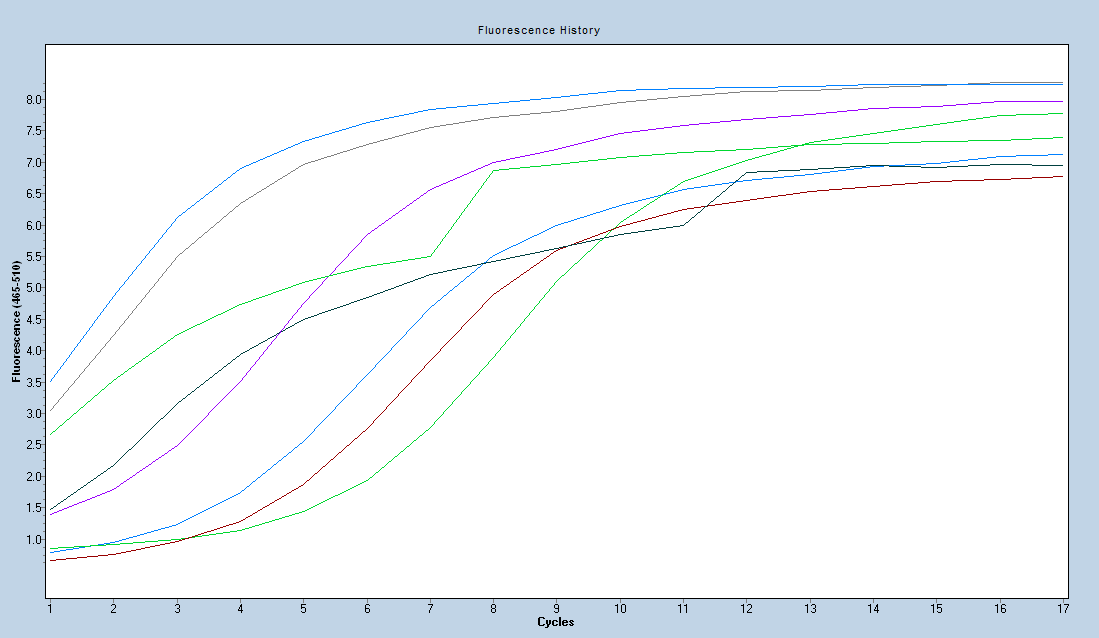
\includegraphics[scale=0.1]{qPCR_D}
    \caption{B}
    \label{fig:qpcr_b}
  \end{subfigure}
  \begin{subfigure}[htpb]{0.3\textwidth}
    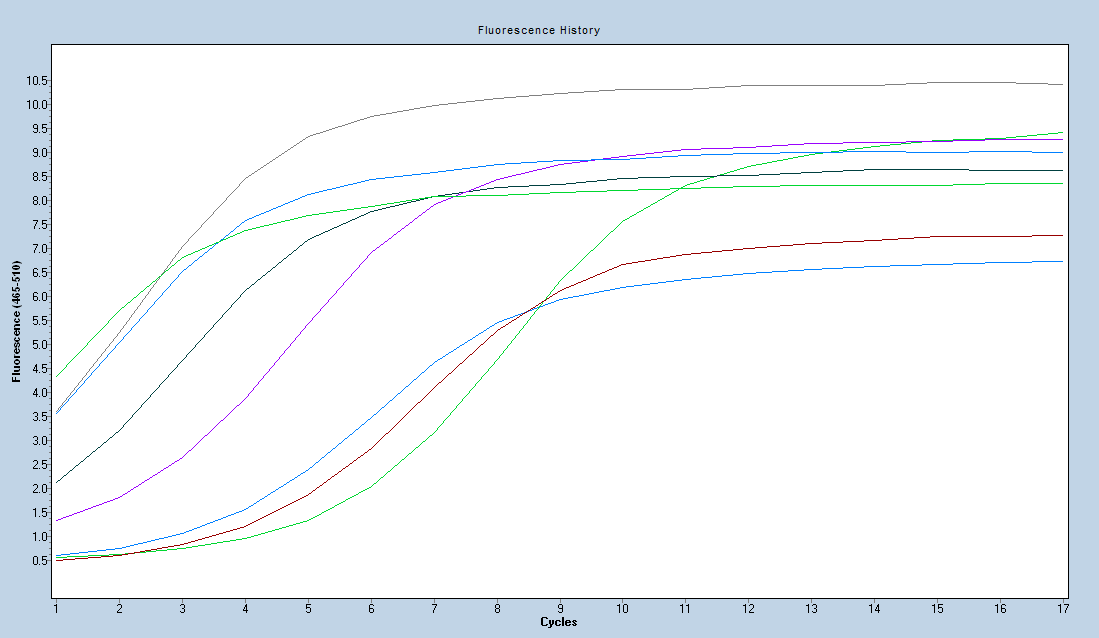
\includegraphics[scale=0.1]{qPCR_F}
    \caption{C}
    \label{fig:qpcr_c}
  \end{subfigure}
  \caption{A - row B, B - row D, C - row H}
  \label{fig:qpcr}
\end{figure}

\subsection{Sequencing}
\label{ssec:emsaselexseq}

Results pending.

\section{PCR Enzyme Bias}
\label{sec:resultenzbias}

Experiments to be done.

\chapter{Discussion}
\label{ch:discussion}

Discussion. 

\chapter{Materials and Methods}
\label{ch:methods}

% Generally too much detail

\section{Nucleosome EMSA SELEX}
\label{sec:metemsaselex}

% Add subsections

The initial DNA ligand is 147 base pairs. This consists of 101 base pairs of random nucleotide sequences flanked by fixed sequences on either side (5$'$ GCTCTTCCGATCT nnnnnnnnnnnnnnnnnnnn AGATCGGAAGAGC 3$'$). This initial DNA ligand was first dissolved in water to yield a \SI{100}{\micro\Molar} solution, then diluted 500-fold in TE buffer with \SI{0.2}{\milli\Molar} EDTA.

% Replace the entire damn thing with a table.
Pre-mixes for PCR amplification were prepared. For `plain' ligands and CpG-methylation, the mix contained 2x Phusion High-Fidelity buffer (ThermoFisher), \SI{0.78}{\milli\Molar} dNTPs (prepared from a \SI{10}{\milli\Molar} dNTP mix), \SI{1.5}{\micro\Molar} forwards primer (5$'$ CCCTACACGAC GCTCTTCC 3$'$), \SI{1.5}{\micro\Molar} reverse primer (3$'$ GCCTTCTCG TGTGCAGAC 5$'$), \SI{4.0}{\micro\Molar} \ce{MgCl2}, and X M Phusion DNA polymerase (ThermoFisher). To create half-C-methylated ligands, the \SI{10}{\milli\Molar} dNTPs were replaced with a \SI{2.5}{\milli\Molar} dNTP mix consisting of dATP, dTTP, dGTP, dCTP, and 5-methyl dCTP in a 1:1:1:0.5:0.5 ratio. To create all-C-methylated ligands, the \SI{10}{\milli\Molar} dNTPs were replaced with a \SI{2.5}{\milli\Molar} mix consisting of dATP, dTTP, dGTP, and 5-methyl dCTP in a 1:1:1:1 ratio.

For each round of SELEX, \SI{25}{\micro\litre} of the respective DNA ligand solution and \SI{25}{\micro\litre} of the corresponding amplification pre-mix were mixed wells in a 96-well deep-well plate. We used a thermocycling protocol modified from that recommended for Phusion High-Fidelity DNA polymerase (ThermoFisher). Thirteen cycles of PCR was followed by ten cycles with the \SI{98}{\celsius} denaturation temperature replaced with \SI{72}{\celsius}.

A pre-mix for CpG-methylation was prepared. This contains 4 U of M.SssI enzyme, \SI{320}{\micro\Molar} S-adenosylmethionine, \SI{7.8}{\milli\Molar} \ce{MgCl2},
and \SI{0.9}{\milli\Molar} DTT. For CpG-methylation, \SI{7.05}{\micro\litre} of this pre-mix was added to \SI{25}{\micro\litre} of the `plain' ligand in 96-well plates, then the mixture was incubated at \SI{37}{\celsius} for 3 hours, followed by \SI{65}{\celsius} for 20 minutes.

\SI{4}{\micro\litre} of a solution of \SI{2}{\Molar} \ce{KCl}, \SI{2}{\milli\Molar} \ce{Mg^{2+}} dissolved in \SI{10}{\milli\litre} TE was dried to each well of a 4ti 384-well plate. Histone octamers were from \emph{Xenopus laevis}. First, the histone octamer concentration was adjusted to \SI{150}{\nano\gram\per\micro\litre} with 1:1 glycerol:refolding buffer (\SI{2}{\Molar} \ce{KCl}, \SI{10}{\milli\Molar} Tris-HCl pH 7.5, \SI{1}{\milli\Molar} Na-EDTA, \SI{5}{\milli\Molar} 2-mercaptoethanol). Then, the histone octamers were serially diluted two-fold to a dilution factor of 16x. To the salted wells of the 384-well plate, \SI{152}{\micro\gram} of the DNA ligand (\SI{4}{\micro\litre} for ‘plain’ ligands, half-C-methylated ligands, and all-C-methylated ligands; \SI{5.2}{\micro\litre} for CpG-methylated ligands) and \SI{1.5}{\micro\litre} of the various dilutions of the histone octamer were added. In a sixth well, refolding buffer was added instead.

% Delete reference to two variants of nucleosome reconstitution
Then, the nucleosomes were reconstituted. Two variants of the nucleosome reconstitution buffer were used for this protocol. One variant was TE buffer with \SI{2}{\milli\Molar} DTT. The other contained TE with \SI{1}{\milli\Molar}, \SI{2}{\milli\Molar} \ce{MgCl2}, and a 6-tab cocktail of protease inhibitor. First, the mixtures were incubated for 30 minutes. Second, \SI{10}{\micro\litre} of the nucleosome reconstitution buffer was added, and the mixture was incubated for 1 hour. Third, \SI{5}{\micro\litre} buffer was added, and the mixture was incubated for 1 hour. Fourth, \SI{5}{\micro\litre} buffer was added, and the mixture was incubated for 1 hour again. Fifth, \SI{70}{\micro\litre} buffer was added, and the mixture was incubated for 1 hour. Finally, \SI{100}{\micro\litre} buffer was added, and the mixture was incubated for 1 hour.

The reconstituted nucleosomes were then run on an EMSA gel. First, the TBE 6\% DNA retardation gel was pre-run at \SI{150}{\volt} with 0.2\% TBE buffer in an ice bath. Then, \SI{10}{\micro\litre} of the reconstituted nucleosome samples (\SI{10}{\micro\litre} sample + \SI{3}{\micro\litre} 5x TBE loading dye) were immediately loaded. The gel was then run at \SI{230}{\volt}, \SIrange{8}{15}{\milli\ampere} per gel for 35 minutes at \SI{4}{\celsius}. Gel bands corresponding to unbound DNA (first lane) and to reconstituted nucleosomes were sliced. The sliced bands were dissolved in \SI{70}{\micro\litre} Tris pH 8.0, and then incubated at \SI{70}{\celsius} overnight. Then, \SI{12.5}{\micro\litre} of this solution was added to \SI{12.5}{\micro\litre} of the corresponding amplification pre-mixes in 96-well plates. SELEX was then performed with a thermocycling protocol modified from that recommended for Phusion High-Fidelity DNA polymerase (ThermoFisher). Here, 21 cycles of PCR with a \SI{98}{\celsius} denaturation temperature and a \SI{67}{\celsius} annealing temperature was followed by ten cycles with a \SI{79}{\celsius} denaturation temperature and a \SI{64}{\celsius} annealing temperature.

Afterwards, the product was CpG-methylated. The resulting ligands then functioned as the input for the next SELEX cycle. In this experiment, four cycles were conducted, and the elutions from the reconstituted nucleosomes were stored.

After all four SELEX cycles, the eluted DNA from EMSA was barcoded for sequencing. This was divided into two experimental sets: one using DreamTaq (ThermoFisher) and one using Phusion DNA polymerase (New England Biolabs). For each set, \SI{9}{\micro\litre} of the eluted DNA was added to \SI{9}{\micro\litre} of PCR mix as recommended by the vendor of each DNA polymerase. To this mixture, \SI{1.5}{\micro\litre} of barcoded PE primer obtained from IDT. Amplification was carried out using the thermocycling protocol recommended for the respective enzyme for 29 PCR cycles.

The results of all 96 wells were pooled for each enzyme. DNA was then purified using 1.2x Ampure beads (Agen Court AMPure). First, 1.2x volume of the beads was added to the pooled DNA sample, and DNA adsorption was allowed to proceed for 5 minutes. Then the beads were precipitated using a magnetic plate. 70\% ethanol was added to wash twice, and the DNA was then eluted with TE buffer (\SI{10}{\milli\Molar} Tris, \SI{0.2}{\milli\Molar} mM EDTA, pH 8.1). The beads were collected by using the magnetic plate again, and the supernatant containing the DNA was pipetted out. It was then diluted to \SI{10}{\nano\Molar}.

\section{PCR Enzyme Bias}
\label{sec:metenzbias}

The input library was lig147. Pre-mixes for PCR amplification were prepared according to manufacturers' specification for the following DNA polymerases: Phire Hot Start II DNA polymerase (ThermoFisher, F122S), Q5 Hot Start High-Fidelity DNA polymerase (New England BioLabs, M0493S), DreamTaq Hot Start DNA Polymerase (ThermoFisher, EP1701), Pfu Turbo DNA Polymerase (Agilent Technologies, 600250), and Phusion High-Fidelity DNA Polymerase (ThermoFisher, F530L). \SI{25}{\micro\litre} of each pre-mix was mixed with \SI{25}{\micro\litre} of the input library, and amplified by thermocycling according to the protocols specified by the manufacturers of each DNA polymerase.

\chapter{Acknowledgements}
\label{ch:ack}

Acknowledgements.

\printbibliography

\end{document}
